\section{Large Scale removal}


\subsection{Zernike polynomials fitting at the aperture}
The Zernike fitting its done in the aperture with the magnitude and phase values. The representation follows the one used in \cite{cassanelli_oof} where the aperture is model as the equation \ref{eq:oof_aperture} where the $B$ term represents the blockage of the telescope, $E(x,y)$ is the illumination and $\phi_z$ represents the large scale errors using the Zernike polynomials as the equation \ref{eq:oof_zernike_errors}, where the $k_{m,n}$ term are the coefficient of each Zernike polynomial.




\begin{equation}
    f(x,y) = B(x,y)E(x,y)e^{i k \phi_z(x,y)}
    \label{eq:oof_aperture}
\end{equation}

\begin{equation}
    \phi_z(x,y) =  \sum_n \sum_m k_{n,m}U^{m}_{n}(\rho, \theta)
    \label{eq:oof_zernike_errors}
\end{equation}


Then for a given radial order $n$ there will be $(n+1)(n+2)/2$ coefficients that needs to be fitted. 
For simplicity we take an uniform illumination and the mask is given by the telescope geometry, with this setup we are only adding 1 more parameter to the optimization process that is the amplitude of the illumination. In principle the illumination function can be changed for any other function, as gaussian or parabolic illumination, but this would add more parameters to the fitting procedure.


The main advantage of using the Zernike fitting is that the contribution of each optical aberration can be separated from the rest and you can determine if the telescope has an optical issue. The drawbacks are that the compuation time is longer than other methods since the optimization process is done in complex values.

\subsection{Polynomial fitting at the surface error}

The second method implemented consists of using a 2D polynomial function composed by the $(x,y)$ coefficients. So for a given order $N$ the function takes the form shown in equation \ref{eq:pol_surf}, where the number of coefficients to be found is $(N+1)(N+2)/2$. 


\begin{gather}
    p(x,y) = \sum_{m=0}^{n-1}\sum_{n=0}^{N-1} c_{n, m} x^{n}y^{m} =\\ 
    c_{00}+c_{10}x+\dots+c_{N0}x^{N-1}+c_{01}y+\cdots+c_{0N}y^{N-1}+c_{11}xy+c_{12}x^1y^2+\cdots
    \label{eq:pol_surf}
\end{gather}

This polynomial fitting is done in the surface of the antenna, so its a real value fitting and its way faster than the Zernike optimization. This surface fitting also considers the blockage of the suporting legs and the subreflector.
The drawback of this method is that you cannot separate the effects of different types of aberrations.


\subsection{Comparison of the methods}

Since both models have similar number of parameters for a given degree (when having uniform illumination the Zernike model has 1 extra parameter compared with the polynomial fitting, the one comming from the illumination) we can compare the fitting results of the two methods. To make a fair comparison the Zernike polynomial result is translated to the antenna surface error. The example map used to compare the methods is the output of the nearfield corrected stage, shown in \ref{fig:nearfield_correction}.
The figures \ref{fig:large_scale_comp_2}, \ref{fig:large_scale_comp_3}, \ref{fig:large_scale_comp_4} and \ref{fig:large_scale_comp_5} shows the comparison of the models generated when removing the large scale errors for different depolynomial degrees. As can be seen the resuults are quite similar and shows the same structures for a given degree. 
For this example the Zernike coefficients with degree 4 are shown in the table \ref{table:zernike_modes}.


\begin{table}[]
    \label{table:zernike_modes}
    \centering
    \caption{Resulting zernike coefficients for the degree=4.}
\begin{tabular}{|l|l|l|}
\hline
Zernike mode & name                         &  value  \\ \hline
n=0,         & Piston                       &  1.25e-5 \\ \hline
n=1,m=-1     & Vertical tilt                &  -5.7e-7 \\ \hline
n=1,m=1      & Horizontal tilt              &  1.2e-5   \\ \hline
n=2,m=-2     & Oblique astigmatism          &  -1.e-5   \\ \hline
n=2,m=0      & Defocus                      &  -2.6e-5   \\ \hline
n=2,m=2      & Vertical astigmatism         &  -7.e-6   \\ \hline
n=3,m=-3     & Vertical trefoil             &  -4.2e-6   \\ \hline
n=3,m=-1     & Vertical coma                &  -1.6e-6   \\ \hline
n=3,m=1      & Horizontal coma              &  4.1e-5   \\ \hline
n=3,m=3      & Oblique trefoil              &  5.1e-6   \\ \hline
n=4,m=-4     & Oblique quadrafoil           &  5.5e-6   \\ \hline
n=4,m=-2     & Oblique second astigmatism   &  -3.7e-6   \\ \hline
n=4,m=0      & Primary spherical            &  3.6e-5   \\ \hline
n=4,m=2      & Vertical second astigmatism  &  -2.4e-6   \\ \hline
n=4,m=4      & Vertical quadrafoil          &  -1.3e-5   \\ \hline
\end{tabular}
\end{table}




\begin{figure}
    \centering
    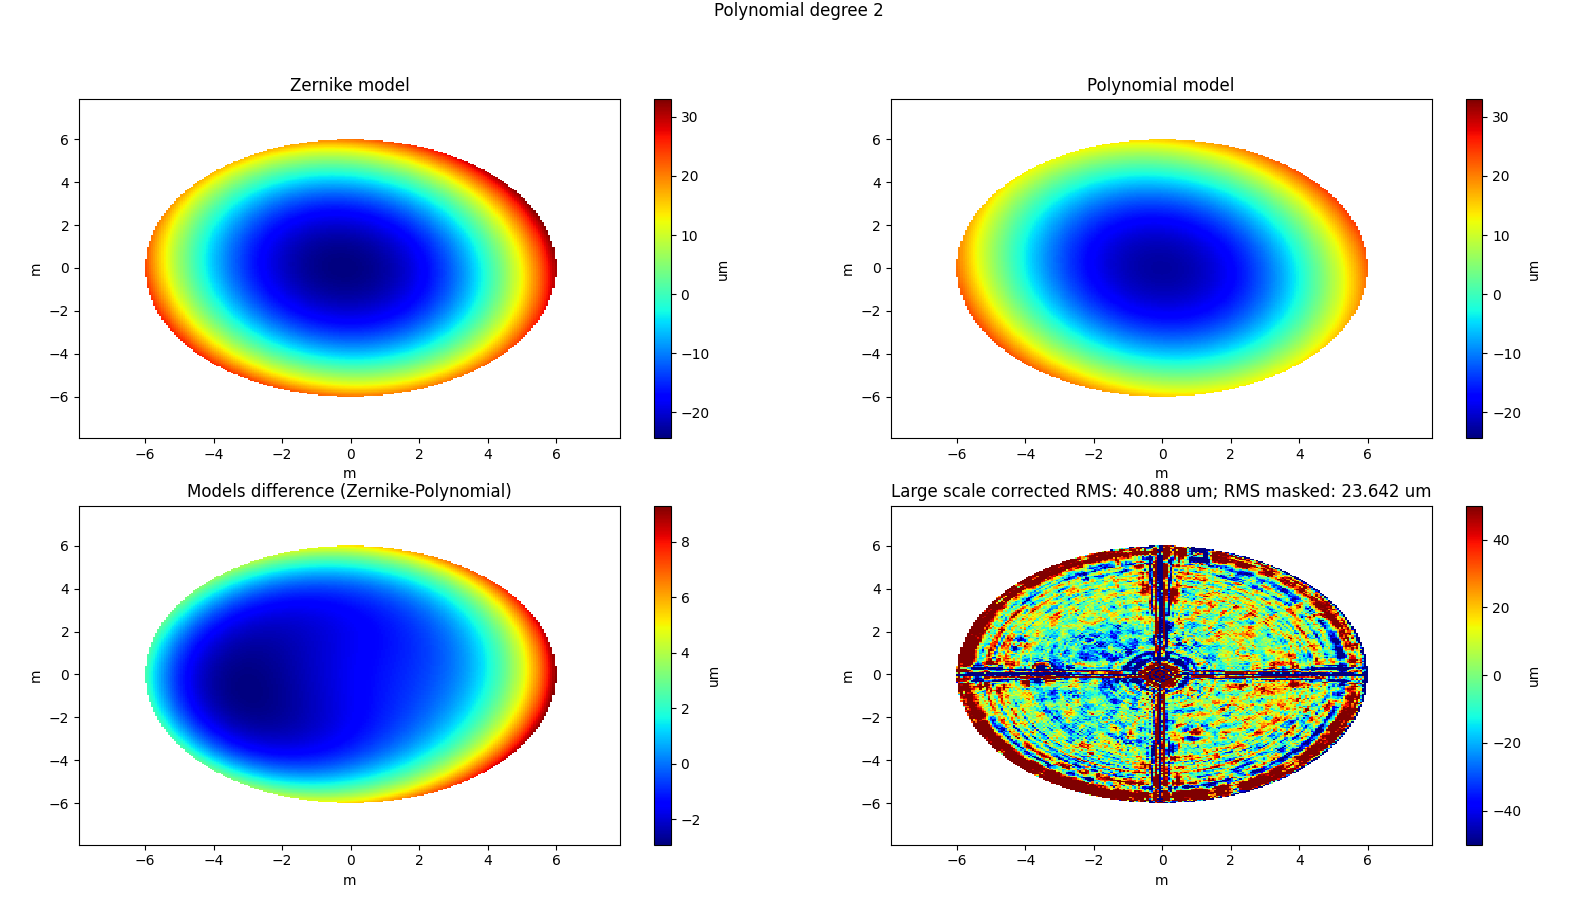
\includegraphics[width=0.9\textwidth]{images/large_scale_comp_2.png}
    \caption{Comparison of both large scale removal methods when using a degree 2 polynomial (6 parameters)}
    \label{fig:large_scale_comp_2}
\end{figure}


\begin{figure}
    \centering
    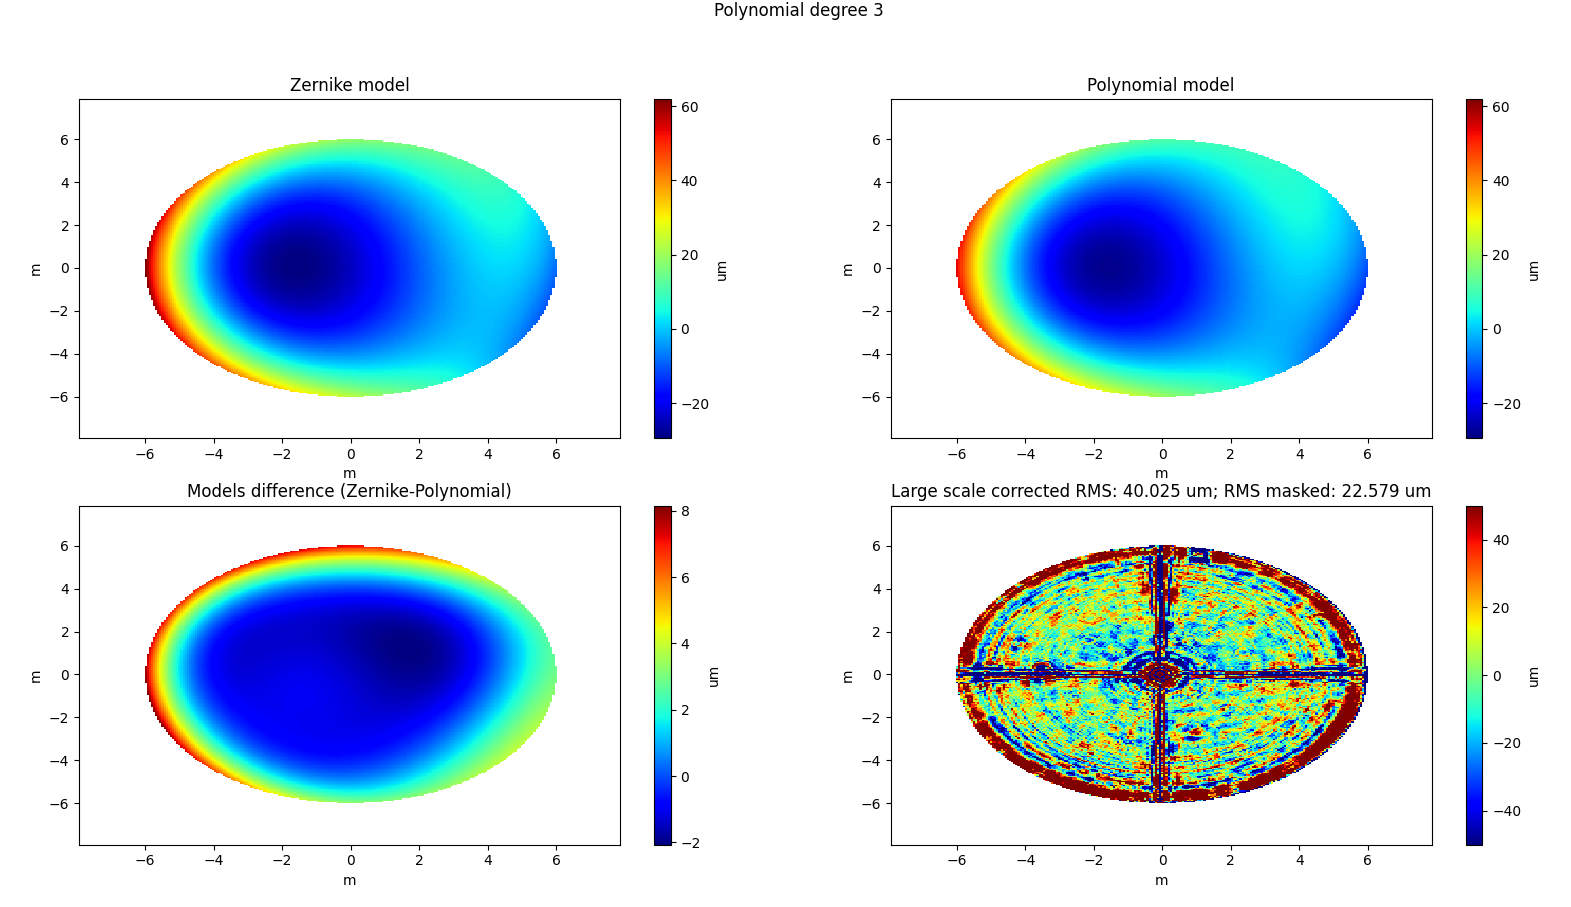
\includegraphics[width=0.9\textwidth]{images/large_scale_comp_3.png}
    \caption{Comparison of both large scale removal methods when using a degree 3 polynomial (10 parameters)}
    \label{fig:large_scale_comp_3}
\end{figure}



\begin{figure}
    \centering
    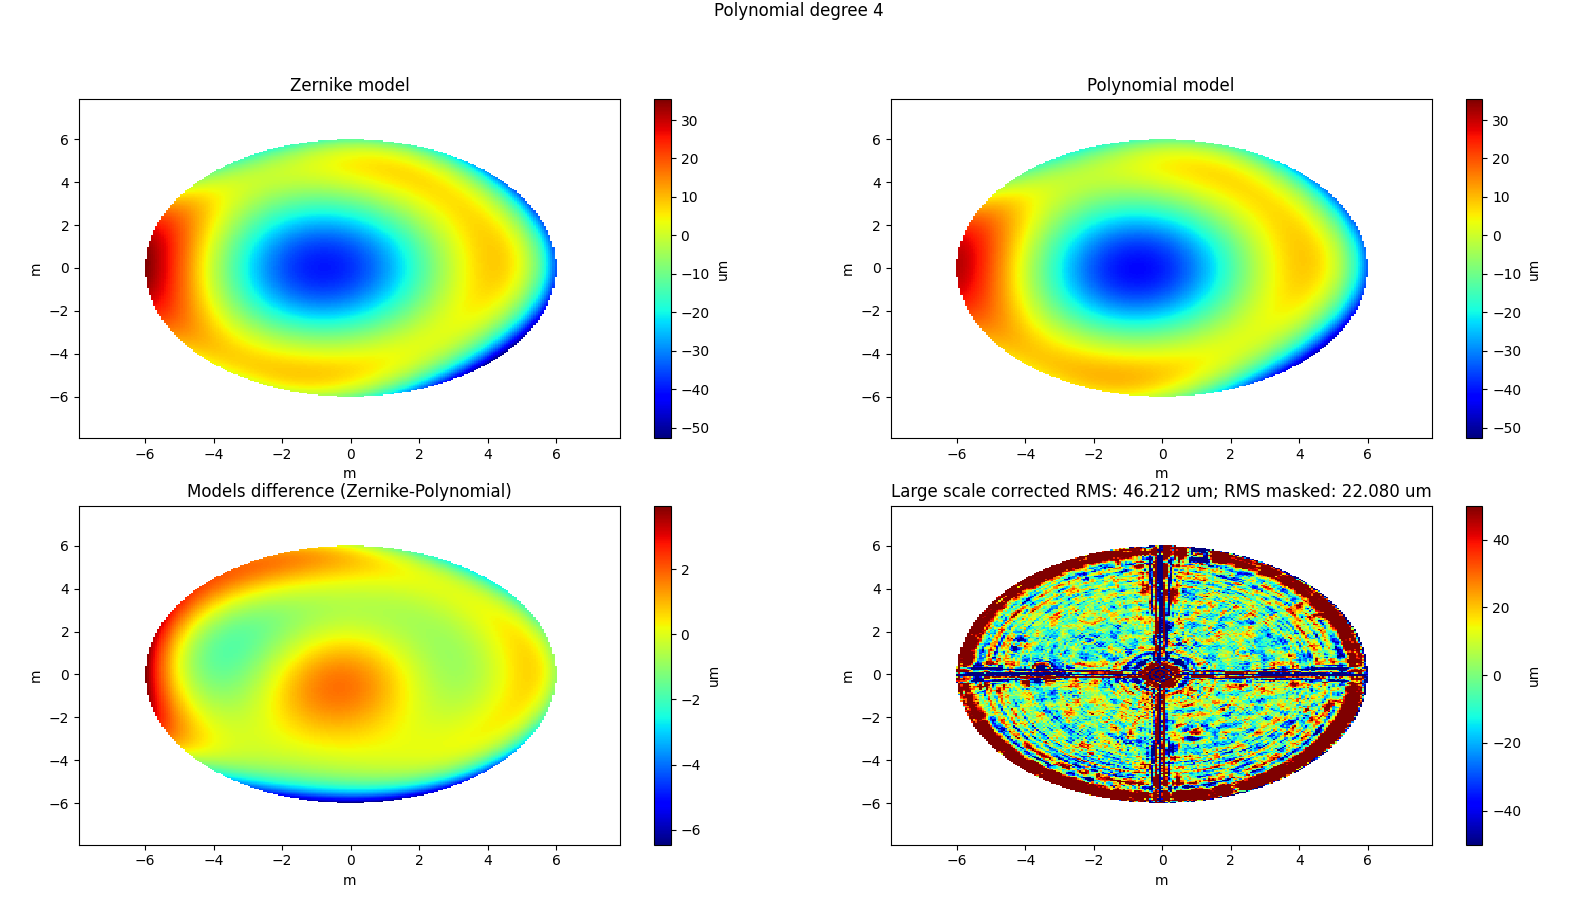
\includegraphics[width=0.9\textwidth]{images/large_scale_comp_4.png}
    \caption{Comparison of both large scale removal methods when using a degree 4 polynomial (15 parameters)}
    \label{fig:large_scale_comp_4}
\end{figure}


\begin{figure}
    \centering
    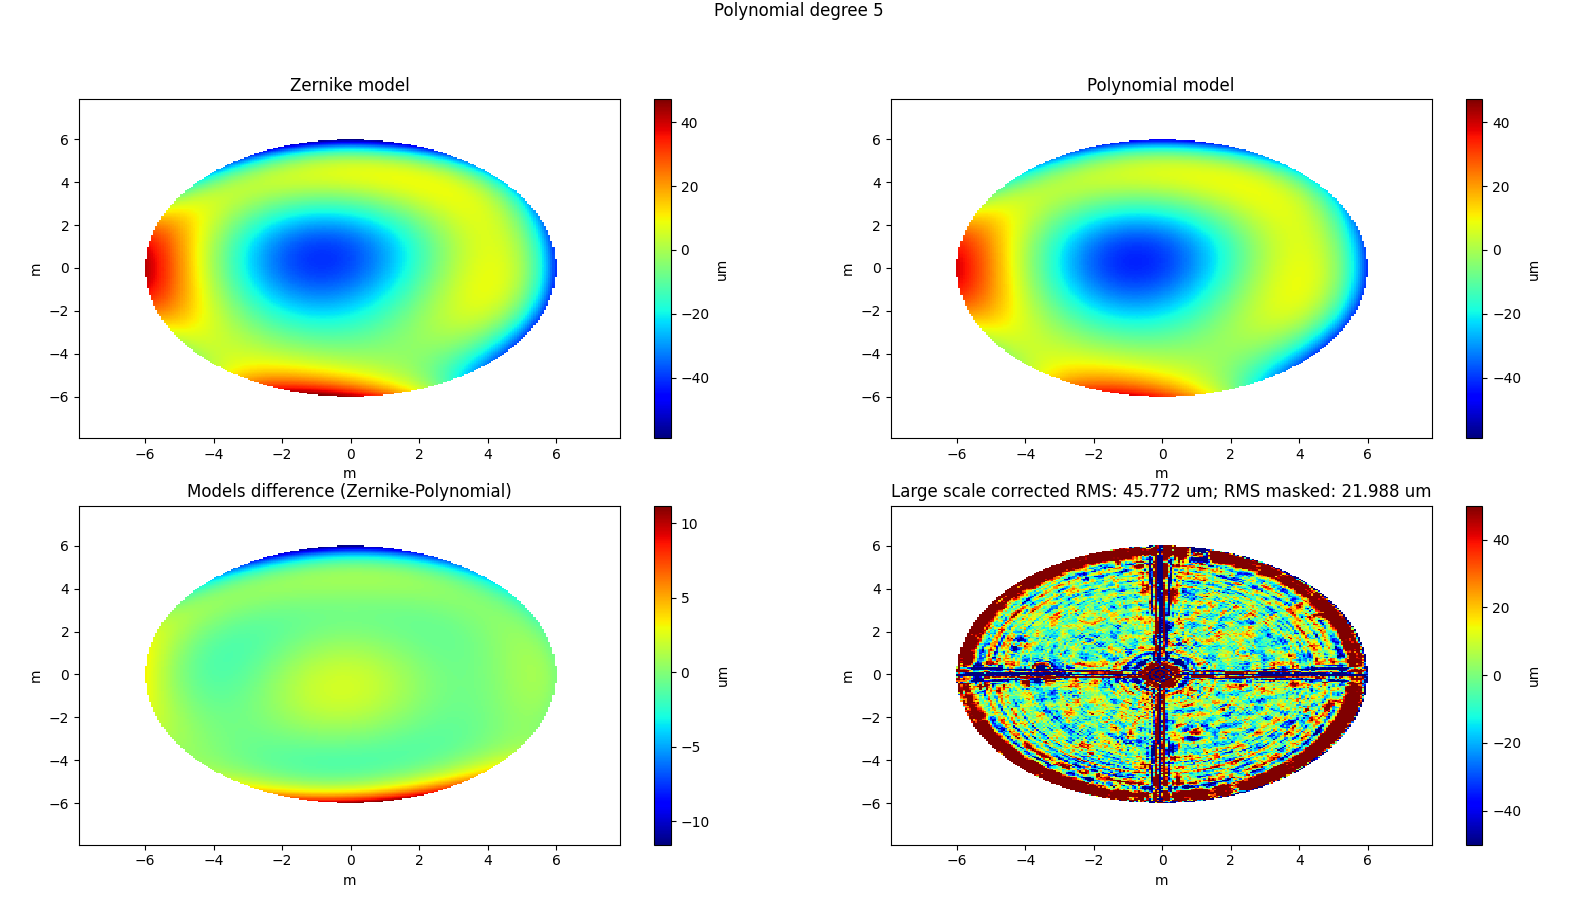
\includegraphics[width=0.9\textwidth]{images/large_scale_comp_5.png}
    \caption{Comparison of both large scale removal methods when using a degree 5 polynomial (21 parameters)}
    \label{fig:large_scale_comp_5}
\end{figure}









